%!TEX TS-program = xelatex
%!TEX encoding = UTF-8 Unicode
%!TeX spellcheck = it_IT
%!TEX root = ../tesi.tex

\chapter{Applicativi}\label{chap:applicativi}
\section{Network Simulator 3}\label{sec:ns-3}
%
% TODO
%
\section{\SUMO}\label{sec:sumo}
\SUMO~\cite{SUMO2012} è un simulatore per traffico veicolare su larga scala; è \textit{open source}, scritto in \Cpp
e distribuito sotto licenza Eclipse Public V2.
Al suo interno si trovano diversi applicativi utili, dall'importazione di dati reali alla creazione di percorsi
per pedoni, diverse tipologie di veicoli, eccetera.
Proprio queste \textit{utility} sono state utilizzate per l'elaborazione delle informazioni sugli edifici (fornite poi
al modello \textit{Obstacle Shadowing}) e il posizionamento dei veicoli.
%
\subsection{Realizzazione degli scenari}
Per creare uno scenario derivato da un ambiente reale, come quelli che saranno utilizzati nelle simulazioni,
e poterlo utilizzare in ns-3, sono necessarie alcune elaborazioni intermedie.

Il primo passo consiste nell'utilizzare la piattaforma gratuita OpenStreetMap (OSM)~\cite{osmWebsite} per
ottenere le informazioni sul mondo reale (Figura~\ref{fig:esempio-file-osm}) e da queste estrarre i dati sugli ostacoli.
Il file ottenuto viene convertito dall'\textit{utiliy} di SUMO Polyconvert che si occupa di tradure alcune informazioni
sugli ostacoli, come per esempio convertire la posizione da coordinate geografiche a cartesiane;
il file risultante conterrà i poligoni che saranno letti dal modulo \textit{Obstacle Shadowing}) (Figura~\ref{fig:esempio-file-poly}).
Il secondo passo è la generazione delle posizioni dei veicoli.
A questo scopo è stato creato uno \textit{script} apposito che, sfruttando le librerie per Python messe a disposizione
nel pacchetto di SUMO, partendo da un punto e percorrendo le strade ammissibili posiziona i veicoli a una certa distanza.
L'articolo originale~\cite{Carpenter:2015:OMI:2756509.2756512} utilizzava una funzione già presente in SUMO
per il posizionamento casuale che però, non permettendo di specificare una distanza fra i veicoli, non andava bene per gli scenari desiderati in questo lavoro.
%
Il file ottenuto dal processo viene convertito in un formato per ns-2 tramite lo \textit{script} traceExporter (sempre compreso nell pacchetto SUMO)
e questo sarà poi eseguito dal modulo di ns-3 \textsf{Ns2MobilityHelper} in modo da posizionare i nodi durante la simulazione.
Il processo completo è riassunto nella Figura~\ref{fig:generazione-file-sumo}.

Il pacchetto SUMO include anche un'interfaccia grafica per visualizzare le simuazion (Figura~\ref{fig:esempio-file-poly}).
% TODO: provare a stampare per vedere come si vedono le immagini !
%
\begin{figure}[htbp]
	\centering
		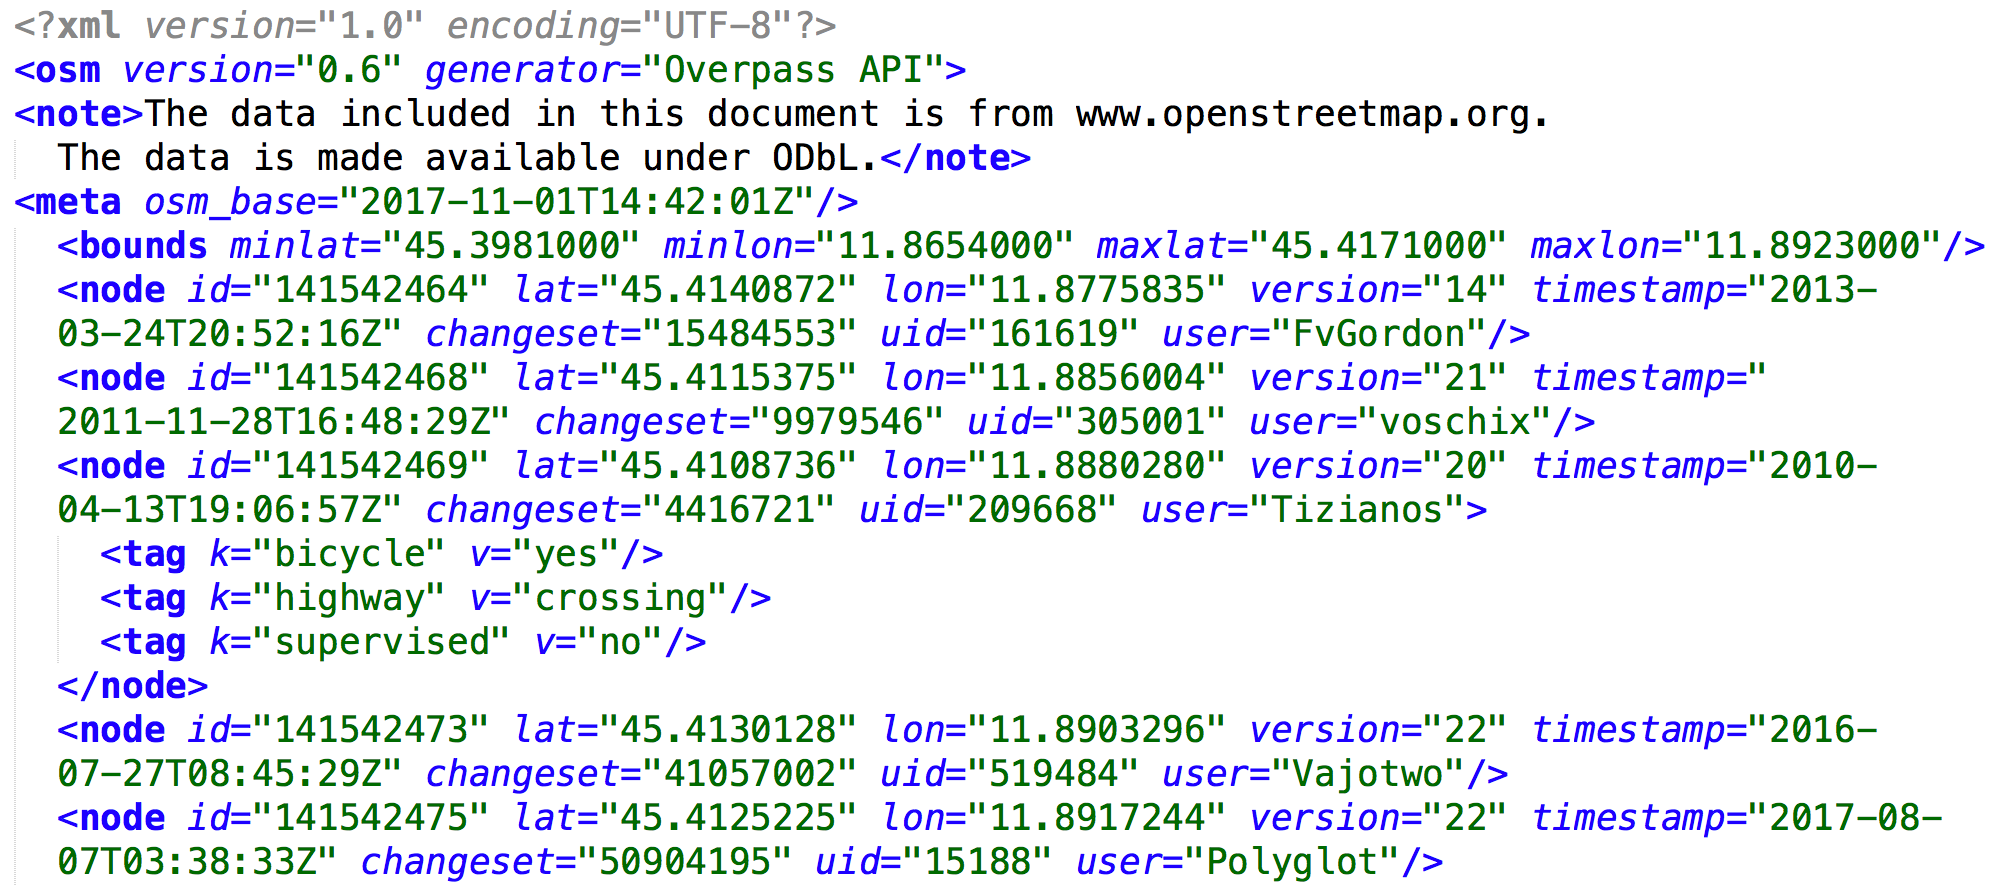
\includegraphics[width=\textwidth]{file-osm-dettaglio.png}
\caption{Un estratto del fle dati sugli edifici dopo la conversione con Polyconvert.\label{fig:esempio-file-osm}}
\end{figure}
%
%
\begin{figure}[htbp]
	\centering
		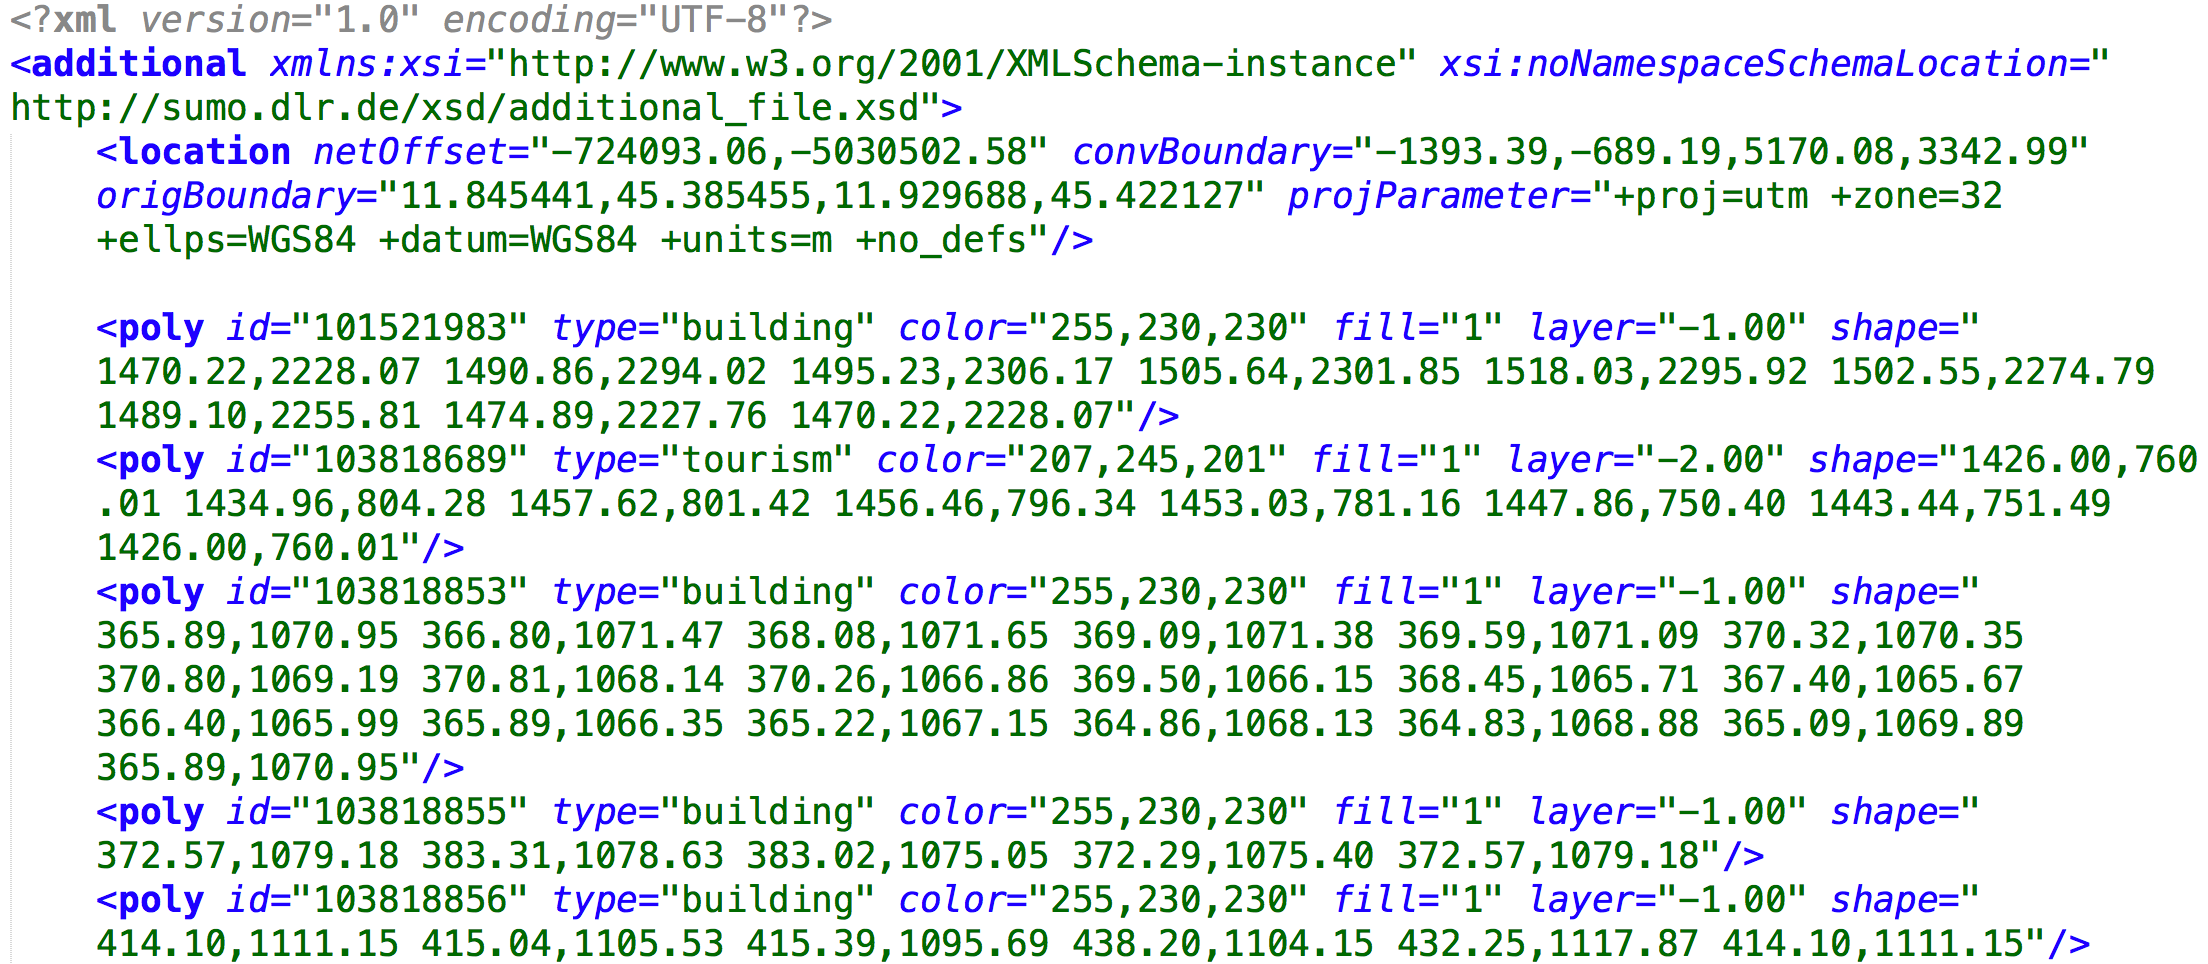
\includegraphics[width=\textwidth]{file-poly-dettaglio.png}
\caption{Un estratto del fle dati sugli edifici dopo la conversione con Polyconvert.\label{fig:esempio-file-poly}}
\end{figure}
%
\begin{figure}[htbp]
	\centering
		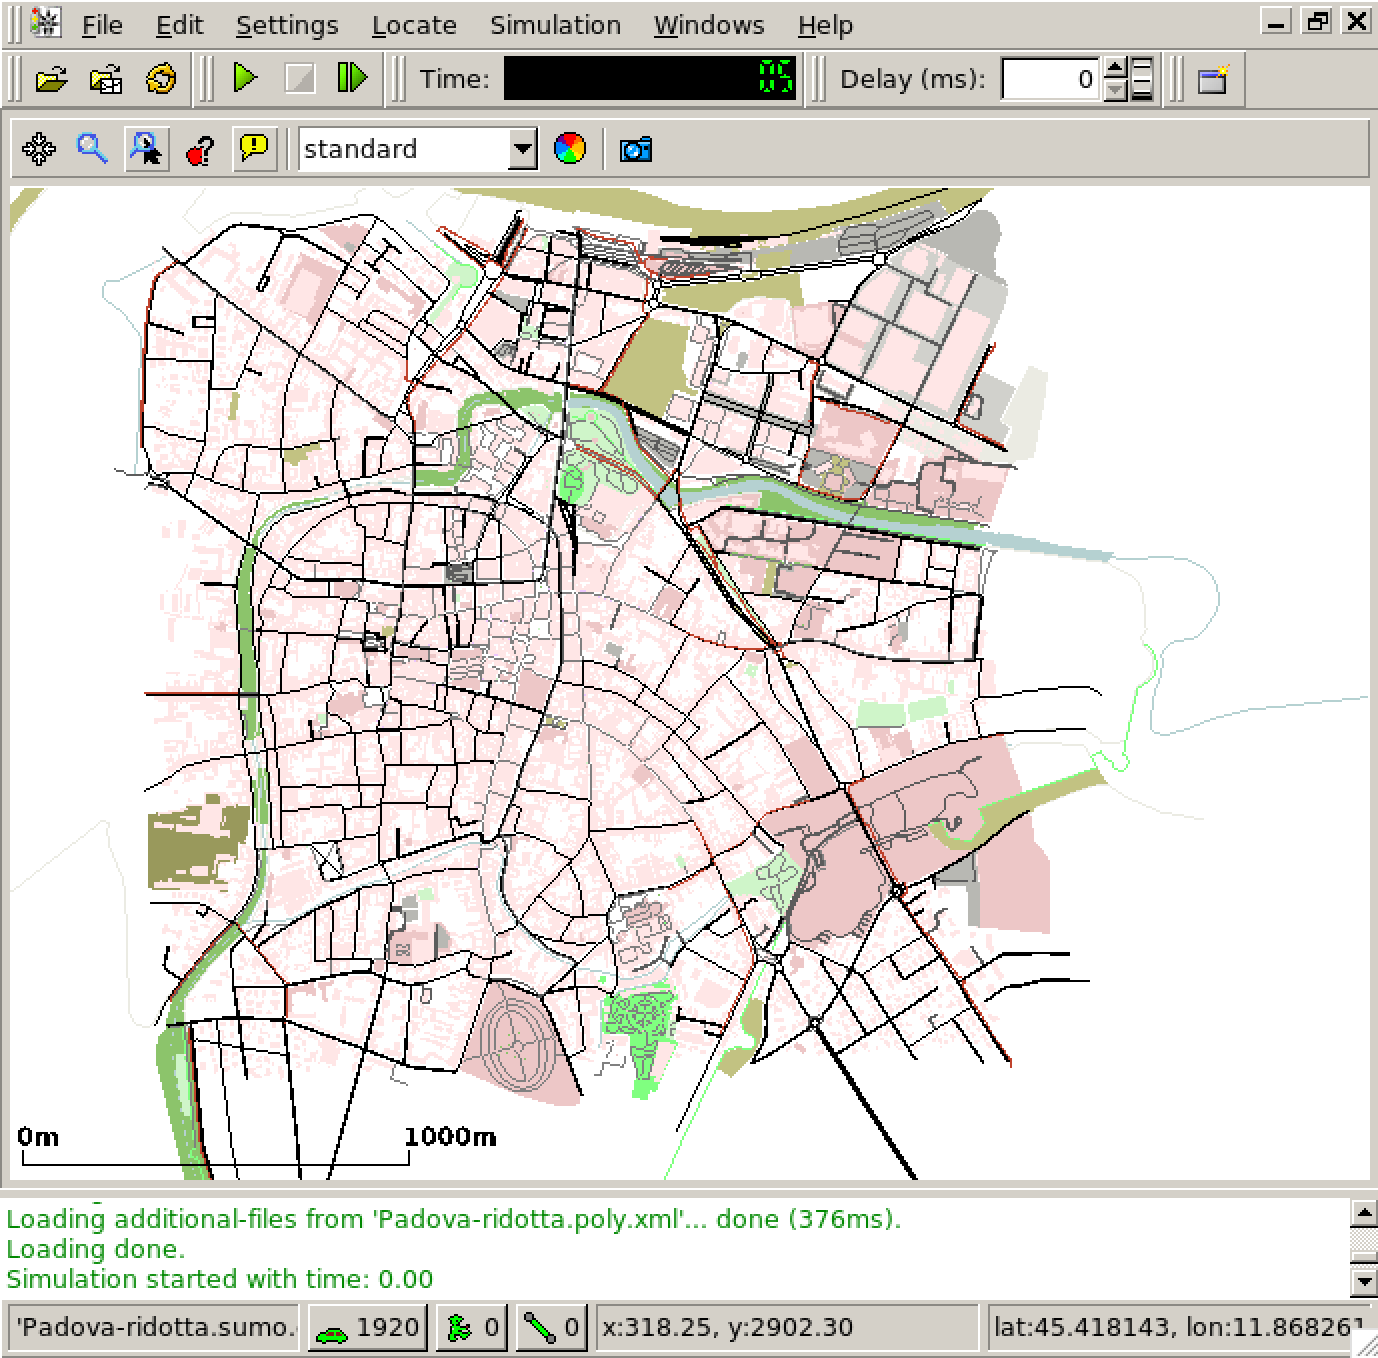
\includegraphics[width=.49\textwidth]{sumo-gui-pd-estesa.png}
		\hfill
		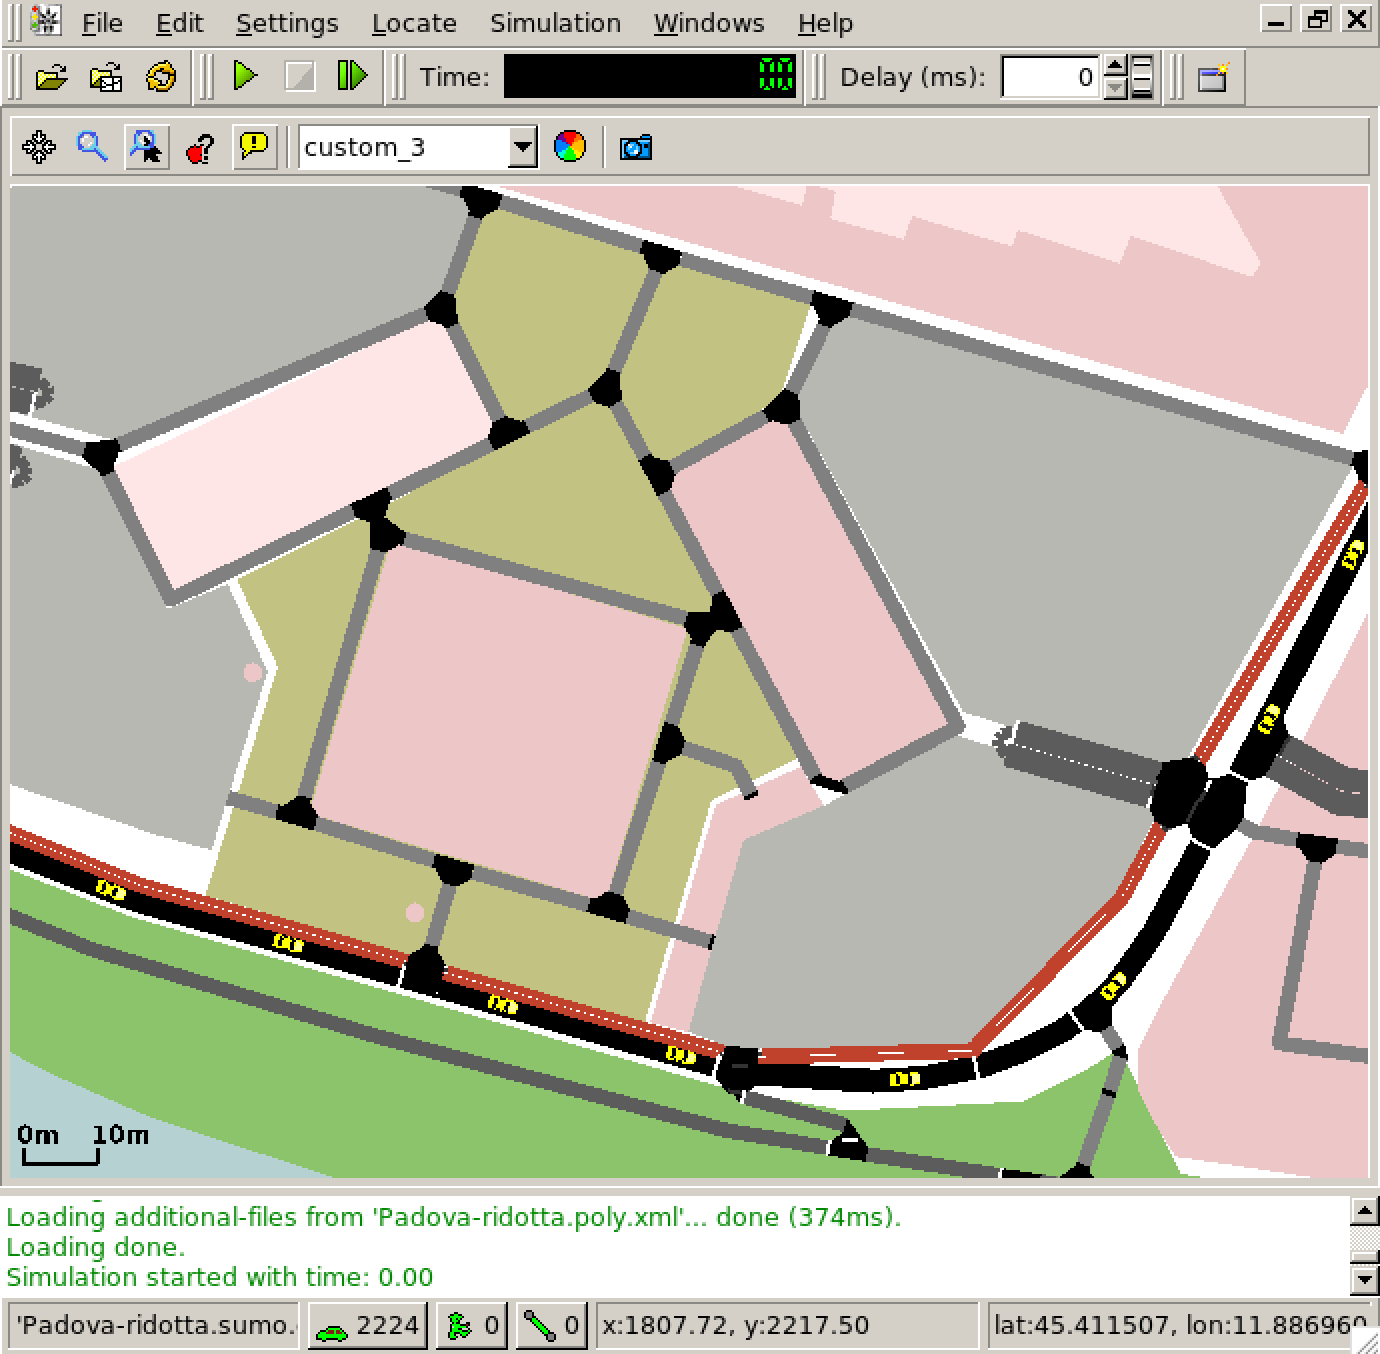
\includegraphics[width=.49\textwidth]{sumo-gui-pd-dettaglio.png}
\caption{Scenario urbano raffigurante il centro di Padova (IT) simulato con SUMO; a destra un dettaglio con i veicoli presenti.\label{fig:sumo-gui}}
\end{figure}
%
% Generazione figura con: https://www.easel.ly/create?id=https://s3.amazonaws.com/easel.ly/all_easels/3240510/1510073603&key=pri
\begin{figure}[htbp]
	\centering
		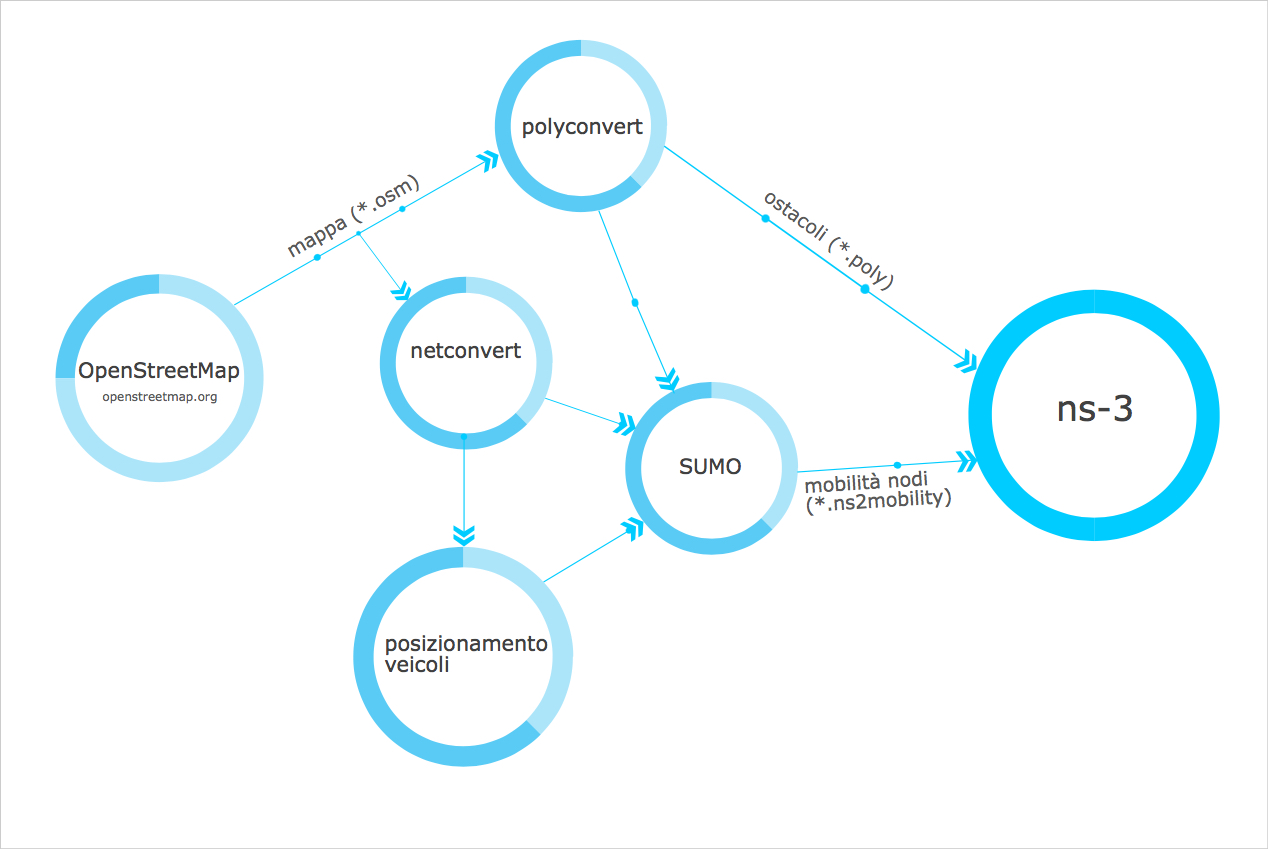
\includegraphics[width=.9\textwidth]{generazione-file-sumo.jpg}
\caption{Procedimento per estrarre le informazioni da OSM e generare i file per la simulazione con ns-3.\label{fig:generazione-file-sumo}}
\end{figure}
